\documentclass[english]{article}
	\usepackage[latin9]{inputenc}
	\usepackage{geometry}
	\geometry{verbose,tmargin=2cm,bmargin=2cm,lmargin=2cm,rmargin=2cm}
	\setlength{\parindent}{0bp}
	\usepackage{mathrsfs}
	\usepackage{amsmath}
	\usepackage{setspace}
	\usepackage{esint}
	\usepackage{marginnote}
	\usepackage{hyperref}
	\usepackage{mathpazo} % font %
	\usepackage{eulervm} % font %
	\usepackage{MnSymbol}
	\usepackage{xcolor}
	\usepackage{outlines}
	\usepackage{graphicx}
	\def\d{\text{d}}
	\def\lap{\Delta}
	\def\id{\text{id}}
	\def\hlf{\frac{1}{2}}
	\newcommand\norm[1]{\left\Vert {#1}\right\Vert }
	\renewcommand\to{\longrightarrow}
	\def\eps{\varepsilon}
	\def\sub{\subseteq}
	\def\subn{\subset}
	\def\C{\mathbf{C}}\def\R{\mathbf{R}}\def\Z{\mathbf{Z}}\def\F{\mathbf{F}}
	\def\disp{\displaystyle}
	\newcommand\floor[1]{\lfloor{#1}\rfloor}
	\graphicspath{ {./imgs/} }
	\newcommand\cyan[1]{{\color{blue}{#1}}}
	\newcommand\orange[1]{{\color{orange}{#1}}}
	\newcommand\red[1]{{\color{red}{#1}}}
	\newcommand\task{\red{Task. }}
	\newcommand{\qed}{$\hfill\blacksquare$}
	\newcommand{\SubItem}[1]{
    	{\setlength\itemindent{15pt} \item[-] #1 }}
	\DeclareMathOperator\End{End}
	\newcommand{\mc}{\mathcal}
	\DeclareMathOperator\img{img}
	\renewcommand{\a}{\mathfrak{a}}
\begin{document}
\section*{1 - A first introduction to prime numbers}
\cyan{Some natural numbers, such as $6=2\cdot 3$, $9=3\cdot 3$, $15=3\cdot 5$, $24=2\cdot 12=3\cdot 8$, $51=3\cdot 17$ and $91=7\cdot 13$ may be decomposed as a product of smaller terms. The remaining numbers, including $1,2,3,5,7,11,13,17,19,\dots,93,97,\dots$ cannot be factored to smaller terms.}
\\\\
Definition. Let $n,k$ be integers, $0<k$. We say $k$ is a factor[divisor] of $n$ if $n=kr$ for some integer $r$. We write this relation as $k\mid n$, and also say $n$ is divisibly by $k$.
\\\\
\cyan{For given $k$, the integers divisibly by $k$ are $0,k,2k,3k,4k,5k,\dots$ as well as $-k,-2k,-3k,-4k,-5k,\dots$.}
\\\\
Understand. We have
\begin{itemize}
\item $1\mid k$ and $k\mid k$.
\item $k\mid r$ and $r\mid n$ imply $k\mid n$.
\item $k\mid n$ and $k\mid m$ imply $k\mid m\pm n$.
\item $k\mid r$ and $n\mid m$ imply $kn\mid rm$.
\item Given any pair of integers $n,k$ with $k>0$, there exists a unique representation $n=kt+s$ with $0\le s<k$.
\item $k\mid n$ implies that either $n=0$ or $k\le |n|$.
\\
\end{itemize} 
\cyan{Decomposing a natural number into a product of factors is analogous to decomposing physical matter into its elements. A water molecule is built of two hydrogen atoms and one oxygen atom, is analogous to $12$ being built of two $2$'s and one $3$, with $12=2\cdot 2\cdot 3$. }
\\\\
Definition. A natural number $p>1$ whose only divisors are one and itself is called a prime number.
\\\\
\cyan{Namely, a prime number is a number one cannot further divide. In formula, $p>1$ is prime if $a\mid p$ implies $a=1$ or $a=p$.}
\\\\
Understand. Each integer $n>1$ can be decomposed as a product of prime numbers (not necessarily different).
\\\\
\cyan{Note that we can factor $24$ in several ways - $2\cdot 12$, $3\cdot 8$, $4\cdot 6$. Continuing to divide all numbers until it is no longer possible, however, we always arrive at the same factorization, $24=2\cdot2\cdot2\cdot3$. To prove the uniqueness of the prime decomposition for all numbers, we first return to the chemistry analogy. When we form a product by mixing two substances in some way, and encounter an atom (a basic element) in the product, then this atom must have come from one of the two substances. In the number world, we have the analogous theorem.}
\\\\
Theorem. If neither of two numbers can be divided by the prime $p$, then their product cannot be divided by $p$ as well.
\\\\
\cyan{The first three prime numbers are $2,3,5$. For $p=2$, the theorem simply states that a pair of odd numbers cannot have an even product. Indeed, any two odd numbers are of the $1+2k,1+2\ell$, with product $1+2(\ell+k+2\ell k)$. For $p=3$, a number not divisible by $3$ is of either form $1+3k$ or $2+3k$. So we have to verify that given two numbers where each is of either of these forms, their product is also in of of these forms. For $p=5$ there's already $4$ options for each form, so $16$ cases we have to check.}
\\\\
Recommendation. Try to find a proof of the theorem by yourself before reading the proof in the next page. Even if it takes a week. I believe in you. All the tools you need are in this page.
\newpage
\cyan{To motivate the proof, say for concreteness sakes $p=97$ and $m=15$. We have $p\mid 15n$, and we want to deduce that $97\mid n$. Write $15n=97k$. Clearly, $3\mid 97k$. We can safely assume (as we are now tackling the case $p=97$ that the theorem holds for the prime $3$, and so $3\mid 97$ or $3\mid k$. But $97$ is prime, so it must be that $3\mid k$. We can then divide both sides of the equation by $3$ to yield $5n=97j$, a similar equation, only $15$ was decreased to $5$. We can do one more step of this argument, now with the prime $5$, to reach the desired $97\mid n$.}
\\\\
Proof. Let $p$ be a given prime number, and \red{suppose the theorem holds for all smaller prime numbers.} Fix a number $n$ for which there exists a number $1\le m$ where $m$ is not divisible by $p$ but $mn$ is divisible by $p$, say $mn=pk$. Our goal is to show that $p\mid n$, namely to show that "$m$ can be replaced with $1$". For this, \red{we shall assume the $m$ we picked is the smallest of all its possible values}. Our goal is to now show that $m=1$. By the minimality of $m$, we have that $m$ is in the range $1,\dots,p-1$. If $m$ were bigger than $1$, then $m$ would have a prime divisor $q$. Moreover, $q$ would be smaller than $p$ (because $m$ is smaller than $p$), so that $q\mid mn=pk$ implies $q$ divides either $p$ or $k$. Of course, $q$ cannot divide the prime $p$, so $q$ divides $k$. Writing $m=qr$, $k=qd$, we have reached the equation $rn=pd$, but now $1\le r < m$ is a contradiction the minimality of $m$. This finishes the proof. \qed
\\\\
\cyan{Let us sketch a second proof. Again, suppose $p=97$ and $m=15$. Then $97\mid 15n$, and we want to deduce that $97\mid n$. We notice it is easier to increase $15$ as follows: we must have $97\mid 30n$, then $97\mid 90n$. But this yields $97\mid 7n$, and we replaced $15$ by the smaller $7$. We can repeat this argument to make the $7$ smaller, etc.}
\\\\
\task Make the above sketch into a rigorous proof.
\\\\
Understand. If $p$ is a prime number and $a_1,a_2,\dots,a_k$ is any sequence of integers with $p\mid a_1a_2\dots a_k$, then $p\mid a_j$ for some $1\le j\le k$.
\\\\
\cyan{The reason $2$ appears exactly $3$ times in the prime factorization $24=2\cdot2\cdot2\cdot3$ is because we can divide $24$ by $2$ three times, but no more. Namely, $24/2=12$, $12/2=6$, $6/2=3$, and $3$ cannot be divided by $2$. More generally.}
\\\\
Definition. Let $n$ be a positive integer and $p$ a prime number. "The number of times $n$ can be divided by $p$" is called the $p$ valuation of $n$ and denoted $\nu_p(n)$. Explicitly, $\nu_p(n)$ is the maximal non-negative integer $k$ for which $p^k\mid n$.
\\\\
Understand. One way to state the above theorem is via the formula $\nu_p(mn)=\nu_p(m)+\nu_p(n)$.
\\\\
Understand. As a corollary of the above theorem, if $n>1$ is an integer which decomposes as a product of (not necessarily distinct) primes $n=p_1p_2\dots p_k$, then for each prime number $p$, the number of times it appears in this factorization is precisely $\nu_p(n)$.


\newpage

\section*{2 - lines and circles}
\cyan{In this chapter, we will see that often, lines and circles are one and the same. This might come as a surprise, and so my first goal to informally convince you that "lines are just circles with infinite radius". We shall give several ways to see this.}
\\
\begin{itemize}
\item Clearly, taking a circle of radius $R$ around the origin and increasing $R$ does not get us close to anything but infinity. But imagine taking a circle passing through the origin, whose center is located at $(0,R)$. Taking $R$ to infinity and standing near the origin, it would appear the circles converge to the $x$ axis.
\href{https://www.desmos.com/calculator/wnpht6jrmp}{Here} is a desmos visualization.
\item Instead of thinking of the circle increasing in size, we may think of a fixed circle, with a perspective on the boundary whose scope is shrinking. The circular arcs (or any smooth arc for that matter) become a line. This is the reason why the spiral milky way galaxy looks approximately straight from earth.
\item In your experience of riding a bicycle or driving a car in a circular path, you may have noticed this can be done by keeping the steering wheel at a constant spot, and not changing your speed. To trace a bigger circular path, the wheel needs to be closer to straight. Of course, a when the wheel is straight, you travel in a straight line.
\item When a point travels at a constant pace around a circle, the direction of its motion is tangent to the circle. \red{If this is surprising to you, or you are not sure what this means, approximate the circle with a perfect $n$-gon inside it, with $n=10^{100}$, and think of the motion there instead.} In total, if the circle had radius $R$ meters and it took us $2\pi R$ seconds to make a full lap, then during those $2\pi R$ seconds the direction of motion changed at a constant pace of $2\pi$ radians per $2\pi R$ seconds, or at $1/R$ radians per second. Taking $R$ to infinity, $1/R$ goes to zero. A motion where the direction in which we are headed does not change is a motion along a straight line.
\item Here is a final argument with physics (or calculus). Imagine again a particle traveling along a circle of radius $R$ meters, at a constant rate, completing a full lap after $2\pi R$ seconds. Then the particle's acceleration is towards the circle's center, at a magnitude of $1/R$ (meter per second squared). Taking $R$ to infinity, $1/R$ goes to zero. A motion with zero acceleration is a motion at a constant pace along a straight line.\\
\end{itemize}
\cyan{We will now discuss some transformations that map circles and lines to each other. The first such map is known as a stereographic projection. Imagine a plane passing containing the equator of the earth. Now imagine that for each point $P$ on earth, except for the north pole $N$, we draw a line from $N$ to $P$. The sterographic projection of $P$ is the intersection of this line with the plane. \href{https://www.desmos.com/calculator/yrlyyh1kvn}{Here} is a desmos visualization in one dimension less.
%Notice that we can extend the stereographic projection continuosly to map the north pole to "the point at infinity". This makes sense, provided that there's one point at infinity, which is reached c in any direction. Under this notion, it makes sense to think of every line (or plane) as containing the point at infinity.
}
\\\\
Understand. Let $\Phi$ be the stereogrphic projection of the sphere to the plane. Show that for every circle $C$ on the sphere passing through the north pole $N$, its image in the plane under $\Phi$ is a straight line. Moreover, this mapping is a bijection between circles on the sphere passing through the north pole and straight lines in the plane.
\\\\
$$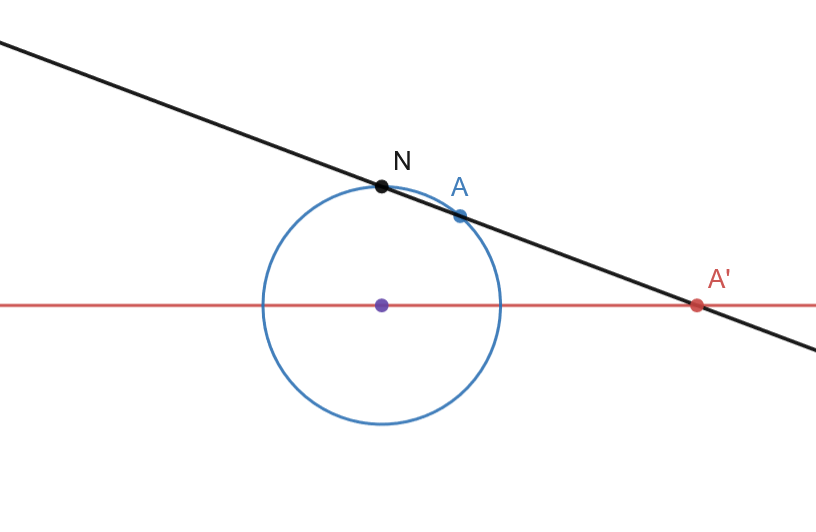
\includegraphics[scale=0.6]{sterographic-projection1.png}$$
\\\\
\cyan{We introduce a concept of "a point at infinity". We think of this point as an added point to $3$-space, which is reached "by traveling an infinite distance, no matter the direction". With this notion, we may extend the definition of the stereographic map so as to send $N$ to $\infty$. Moreover, we think of $\infty$ as being included in every line, and in every plane. In particular, parallel lines in the plane now intersect - at $\infty$. Similarly, non-parallel lines in the plane intersect at two points.}
\\\\
\cyan{Our next goal is to show that the sterographic projection maps circles not through $N$ to circles in the plane bijectively. This can be bashed out with formulas, but the path we'll take to this result is one Euclid could have walked.}
\\\\
Understand. The stereographic projection $\Phi$ has the following property: $NA\cdot NA'=2$ where $A'=\Phi(A)$.
\\\\
\cyan{The above property allows us to extend the stereographic projection to not be defined only on the sphere, but the entire $3$-space.}
\\\\
Definition. An inversion $\Phi$ (in $d$-space, centered at a point $N$, with positive constant $c$) is the mapping that takes each regular point $A$ to the point $A'$ on the ray from $N$ through $A$ for which $NA\cdot NA' = c$. For the two nonregular points $N$ and $\infty$, the inversion swaps them.
\\\\
Understand.
\begin{itemize}
\item The stereographic projection is the restriction of the inversion in $3$-space through $(0,0,1)$  with constant $2$.
\item In $\C$, the inversion at $0$ with constant $1$ is given by $z\mapsto 1/\bar{z}$.
\item $\Phi$ is an involution. Namely if $\Phi$ maps $A$ to $A'$, then it also maps $A'$ to $A$.
\item The fixed points of $\Phi$ form the sphere centered at $N$ with radius $\sqrt{c}$.
\item If $A,B$ are regular, then $NAB\sim NB'A'$.
\begin{outline} 
\item $\Phi$ maps spheres/hyperplanes to spheres/hyperplanes. More precisely:
\1 If $P$ is a hyperplane through $N$, then $\Phi(P)=P$.
\1 If $S$ is a sphere centered at $O$ not passing through $N$, then $\Phi(S)$ is the sphere with diameter $B'A'$ where $\{A,B\}$ is the intersection of the line $\ell(N,O)$ with $S$.
\1 If $S$ is a sphere with diameter $NA$, then $\Phi(S)$ is the plane through $\Phi(A)$ orthogonal to $NA$.
\1 Conversly, if $P$ is a hyperplane not containing $N$, then $\Phi(P)$ is a sphere through $N$.
\end{outline}
\item Finally, the sterographic projection maps circles not through $N$ to circles in the plane bijectively.
\\
\end{itemize} 
\cyan{In $\C\cup{\infty}$, let us circles and lines clines. Under the sterographic bijection with the unit sphere, clines in $\C\cup{\infty}$ correspond simply to circles in the sphere.}
\\\\
Understand. For each three (distinct) points $A,B,C\in \C\cup\infty$, there is a unique cline containing them.
%Since $z\mapsto 1/\bar{z}$ is a bijection of clines, so is $I:z\mapsto 1/z$. But so is every $H:z\mapsto az+b$ for all $a,b\in \C$, $a\neq0$. It follows that any composition of these maps acts as a bijection of clines.}

%Understand. The group $M$ of bijections of $\C\cup\infty$ of the form $z\mapsto \dfrac{az+b}{cz+d}$ is precisely the group generated by 


\newpage
%%%	%%%	%%%	%%%	%%%	%%%	%%%
%%%	%%%	%%%	%%%	%%%	%%%	%%%
%%%	%%%	%%%	%%%	%%%	%%%	%%%
			\section*{100 - modules over a polynomial ring}


\cyan{Motivation.} An $\R$ module is simply a real vector space. A $\Z$ module is simply an abelian group. What is an $\R[t]$ module? What is a $\Z[t]$ module?	\\\\


\orange{Understand.} Given a ring $A$, we have a natural bijection between $A[t]$ modules $\mc{M}$ and pairs $(M,T)$ where $M$ is an $A$ module and $T\in\End_A(M)$.	\\\\


\orange{Exercise.} Under the above correspondence, what do submodules of an $A[t]$ module correspond to? What do homomorphisms correspond to?	\\\\


\cyan{Trick.} When we have an algebra problem with data $M,T\in\End(M)$, we instead get an equivalent algebra problem with data $M$, just now working over $A[t]$. \\\\


To convince you of the power of this trick, we shall now present two nontrivial applications.		\\\\


Theorem 1. Given $T\in\End_A(M)$, we have  $T^r+a_1T^{r-1}+\dots+a_r\id = 0$ for some $a_1,\dots,a_r\in A$, under the assumption that $M$ has a generating set of order $r$.	\\\\


Theorem 2. Given $T\in\End_A(M)$, we have $T$ surjective $\implies$ $T$ bijective (and moreover its inverse is a polynomial in $T$), under the assumption that $M$ is finitely generated.		\\\\


\newpage


Proof of theorem 1. Let $M$ be generated by $m_1,\dots,m_r$. We pick entries $\psi_{ij}\in A^{r\times r}$ for which $Tm_i=\sum\psi_{ij}.m_j$. Now consider $M$ as an $A[t]$ module via $f(t).m=f(T)(m)$. Then for $\Psi=t\id_r-\psi \in A[t]^{r\times r}$ we have $\Psi.\left(\begin{array}{c}
m_{1}\\
\vdots\\
m_{r}
\end{array}\right)=\left(\begin{array}{c}
0\\
\vdots\\
0
\end{array}\right)$.
Recall that (by multiplying by the adjoint) this implies $\det\Psi$ annihilates $m_1,\dots,m_r$. However, $\det\Psi=f(t)$ is simply a monic polynomial in $t$ of degree $r$, and we get our desired $f(T)=0$.	\\\\


Proof of theorem 2. We start similarly to our proof of theorem 1. Only now we pick entries $\phi_{ij}\in A^{r\times r}$ for which $m_{i}=\sum\phi_{ij}.Tm_{j}$. For $\Phi=\phi_{ij}t-\id_{r}\in A[t]^{r\times r}$ we have $\Phi.\left(\begin{array}{c}
m_{1}\\
\vdots\\
m_{r}
\end{array}\right)=\left(\begin{array}{c}
0\\
\vdots\\
0
\end{array}\right)$, and so $\det\Phi$ annihilates $m_1,\dots,m_r$. However, $\det\Phi=g(t)$ is a polynomial in $t$ with constant coefficient $\pm 1$, and we have $g(T)=0$.	\\\\


\orange{Exercise.} Extend theorem 1, by showing that if $\img T\le \a.M$ for some ideal $\a$, then we can make it so $a_i\in \a$.	\\\\


\orange{Exercise.} Deduce theorem 2 from the above extension of theorem 1.
%Solution. Work over $A[t]$, let the endomorphism be the identity, and the ideal $(t)$.






\end{document}
